%%%%%%%%%%%%%%%%%%%%%%%%%%%%%%%%%%
%%%%%%%%%%%%%%%%%%%%%%%%%%%%%%%%%%
%Template for the ``TFM''
%%%%%%%%%%%%%%%%%%%%%%%%%%%%%%%%%%
%%%%%%%%%%%%%%%%%%%%%%%%%%%%%%%%%%%%%%%%%%%
\documentclass[aps,pra,twocolumn,10pt,floatfix]{revtex4-2}
%%%%%%%%%%%%%%%%%%%%%%%%%%%%%%%%%%%%%%%%%%%
\usepackage{graphicx,epsfig}
\usepackage{amsmath}
\usepackage{amsfonts}
\usepackage{fancyhdr}
\usepackage{listings}
\usepackage{hyperref}
	\hypersetup{
    colorlinks=true,
    linkcolor=blue,
    filecolor=blue,      
    urlcolor=blue,
    }

\usepackage{lipsum}


%%%%%%%%%%%%%%%%%%%%%%%%%%%%%%%%%%%%%%%%%%%
%%%%%%%%%%%%%%%%%%%%%%%%%%%%%%%%%%%%%%%%%%%

% Here you must introduce the following information:

% Title of the TFM
\def \TFMtitle {Template for the TFM report}

% Student's name
\def \student {Your Name Here}

% Student's email
\def \emailaddress {your.name.here@ub.edu}

% Master's email
\def \mdemailaddress {master.complex.biophys@ub.edu}

% Advisor's name
\def \advisor {Ada Lovelace}

%%%%%%%%%%%%%%%%%%%%%%%%%%%%%%%%%%%%%%%%%%%
%%%%%%%%%%%%%%%%%%%%%%%%%%%%%%%%%%%%%%%%%%%

\begin{document}

%%%%%%%%%%%%%%%%%%%%%%%%%%%%%%%%%%%%%%
\pagestyle{fancy}
\lhead{\bf The title, shortened if needed}
\rhead{\student}
%%%%%%%%%%%%%%%%%%%%%%%%%%%%%%%%%%%%%%


\title{\TFMtitle}
%
\author{Author: \student}
\email{\emailaddress} 
\affiliation{Master en F\'{\i}sica dels Sistemes Complexos i Biof\'{\i}sica.\\ Facultat de F\'{\i}sica, Universitat de Barcelona, Mart\'{\i} i Franqu\`{e}s 1, 08028 Barcelona, Spain.}
\email{\mdemailaddress} 
%
\author{Advisor: \advisor}
\affiliation{You may have more than one advisor, and you can introduce additional information about them.\\Institution/Company X, Street Y, City Z.}
%
\date{\today}

\begin{abstract}
{\bf Abstract:} This is a simple document created with \LaTeX that you must use as a template for your TFM report document.
Some examples of the use are also given in this template. 
First instruction: The report must begin with an abstract of {\bf up to 500 words}.
\end{abstract}

\maketitle

%\tableofcontents
% the command above can be uncommented if you want to show a table of contents

%%%%%%%%%%%%%%%%%%%%%%%%%%%%%%%%%%%%%%%%%%%%%%%%%%%%%%%%%%%%%%%%%%%%%%%%%%%
\section{Introduction}

This document is the template you must use when preparing your TFM report. The length of the report must be between {\bf 12 and 16 two-column pages}, excluding the bibliography, the acknowledgments and the appendices. Otherwise the essay will not be considered for evaluation, and will automatically fail.
The report must have the format (structure, minimum and maximum length, pagination, etc.) of the present template, and must be written in (good) English.

The report must begin with an abstract of up to 500 words, include an introduction and a conclusion section, and references must be cited with the IEEE style. You can find the bibliography style guidebook at \url{https://ieeeauthorcenter.ieee.org/wp-content/uploads/IEEE-Reference-Guide.pdf}.

The evaluation of the subject takes into account the advisor's and the jury's evaluations. 
The {\it Assessment Rubrics} will be available at the virtual campus, and it is highly advisable for the students to read them thoroughly and carefully. 
The final qualification will measure the assessment of your merits corresponding to the completion of the project (20 \%), the writing of the report (40 \%) and the presentation of the results (40 \%).

The public defense of the TFM consists of an oral presentation of 20 minutes, followed by a round of questions from the jury of a maximum of 15 minutes. In this oral presentation, English is compulsory, at least in the discussion with the jury. Students who opt for the maximum qualification of MH may be called by the master's coordination committee to a second oral defense of 10 minutes entirely in English followed by another 10 minutes of questions of the jury. 


%%%%%%%%%%%%%%%%%%%%%%%%%%%%%%%%%%%%%%%%%%%%%%%%%%%%%%%%%%%%%%%%%%%%%%%%%
\section{Equations: a few examples}

Lets start writing some equations, There are several ways to enter formulas. We can enter them on the same line, like the Boltzmann equation: $S=k_B\ln\Omega$, or in a separate line, like the Sch\"{o}dinger equation: $$i\hbar\frac{\partial}{\partial t}\Psi(\vec{r},t) = \hat{H}\Psi(\vec{r},t),$$ or listed with a label so that we can refer to them later. For instance you can refer to it as Eq.~(\ref{partition}):
\begin{equation}
\oint_{\partial \Sigma}\vec{B}\cdot d\vec{l} = \frac{1}{c}\left(4\pi\iint_{\Sigma}\vec{J}\cdot\vec{S}+\frac{d}{dt}\iint_{\Sigma}\vec{E}\cdot d\vec{S}\right),
\label{partition}
\end{equation}
which is Amp\`{e}re's law.

If your equations are too long you can divide them in multiple lines as seen in Eq.~(\ref{longeq}),
\begin{multline}
p(x) = ax^6 + bx^5y + cx^4y^2 + dx^3y^3\\ 
- ex^2y^4 - fxy^5 + gy^6 - h^3b^3.
\label{longeq}
\end{multline}
Also you can introduce aligned equations:
\begin{align} 
\nabla {\cdot} \vec{E}&= 4 \pi \rho, \label{maxwell1}\\
\nabla \times \vec{B} - \frac{1}{c} \frac{\partial \vec{E}}{\partial t} &=
\frac{4 \pi}{c} \vec{J}, \label{maxwell2}\\
\nabla \times \vec{E} +\frac{1}{c} \frac{\partial \vec{B}}{\partial t} &=
0, \label{maxwell3}\\
\nabla {\cdot} \vec{E}&= 0.
\label{maxwell4}
\end{align}
You can find Eqs.(\ref{maxwell1}), (\ref{maxwell2}), (\ref{maxwell3}), and (\ref{maxwell4}) in Ref.~\cite{jackson}.

Finally you can display different cases, as it is needed for the case of the Heaviside function:
\begin{equation}
 u(x) =
  \begin{cases}
   0,        & \text{if } x \geq 0, \\
   1,        & \text{otherwise}.
  \end{cases}
\end{equation}

Do not forget to use punctuation in the displayed equations.


\subsection{Tables and figures}

Sometimes you will need to insert a table with data. Below, in Table~\ref{tab:constants}, you will find an example of a table.
%
\begin{table}[h]
 \centering
 \caption{Physical constants.}
\label{tab:constants}
\vspace{2mm}
\begin{tabular}{c c c}
\textbf{} & \textbf{Symbol} & \textbf{Value}\\\hline\hline
Speed of light & \textit{c} & $3\times 10^{8}$ m/s\\\hline
Planck's constant & \textit{h} & $6.6 \times 10^{-34}$ J s\\\hline
Electron charge & \textit{e} & $1.6\times 10^{-19}$ C\\ \hline\hline
\end{tabular}
\end{table}
%

The data you collect in the lab, obtained by numerical simulations, and/or processed at home will be showed with graphics, or even better, we can decide to show a picture of Richard P. Feynman playing the bongos as in Fig.~\ref{feynman}.
%
\begin{figure}[b]
  \centering
  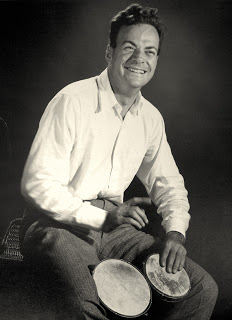
\includegraphics[scale=0.45]{feynmanbongos.jpg}
  \caption{R. P. Feynman solving integrals.}
  \label{feynman}
\end{figure}
%
But now seriously, figures showing data must look like Fig.~\ref{data}.
%
\begin{figure}
  \centering
  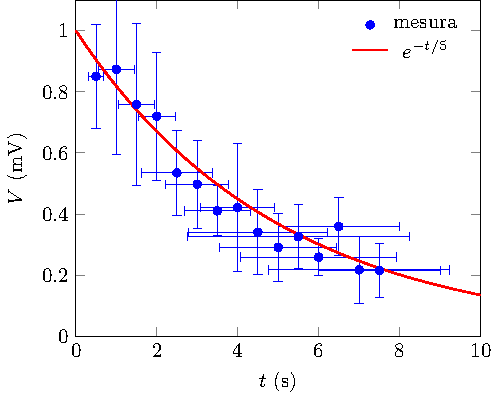
\includegraphics[width=\columnwidth]{figure.pdf}
  \caption{A nice plot. Plots showing your data must contain labeled axes with font sizes large enough to be read (as the one shown here). Data points should be clear and differentiate in case you plot different sets in the same plot (use different shapes and colors). Captions must contain a short description of what the figure depicts. The discussion must be developed in the main text.}
  \label{data}
\end{figure}
%
For this you need, of course, to have created the figure before, in this case figure.pdf file.


%%%%%%%%%%%%%%%%%%%%%%%%%%%%%%%%%%%%%%%%%%%%%%%%%%%%%%%%%%%%%%%%%%%%%%%%
\section{Developing sections}

Sometimes in your report you will need to itemize. Here you have an example:
%
\begin{itemize}
	\item First item.
	\item Second item.
	\item And so on\dots
\end{itemize}
%
Or maybe an enumeration of facts:
%
\begin{enumerate}
	\item First item.
	\item Second item.
	\item And so on\dots
\end{enumerate}

\lipsum[1-2] %dummy text to fill space. This is only for displaying purposes. Remove from your working document


\subsection{Subsection 1}

\lipsum[5-6]

\subsection{Subsection 2}

\lipsum[7-9]



\section{Conclusions}

Your report must include a Conclusions section.

\textbf{Here ends the page counting!}
\\

\section*{Appendix}

If we want to add complementary information such as the explanation of a mathematical algorithm or the code written to analyze the data, we will do so in this space.

\subsection{One example of an Appendix}

For instance, if we want to introduce a code we will do it using the \verb listings! package.

\begin{lstlisting}
import numpy as np
    
def incmatrix(l1,l2):
    m = len(l1)
    n = len(l2)
    M = np.zeros((n*m,1), int)  

    for i in range(m-1):
        M[(i)*n] = 1;
    return M
\end{lstlisting}


\begin{acknowledgments}
Be sure to thank everyone who help during your TFM: your advisor, your colleagues, and granting agencies if it is the case.
\end{acknowledgments}


\begin{thebibliography}{99}

\bibitem{book}H. Kopka and P.W. Daly, \textsl{A Guide to
\LaTeX: Document Preparation for Beginners and Advanced Users}, 3rd. ed. Reading, MA, USA: Addison-Wesley, 1999.

\bibitem{footnotes} It is necessary to process a file twice to
get the counters correct.

\bibitem{jackson} J.D. Jackson, {\it Classical Electrodynamics}, 2nd. ed. New York, NY, USA: John-Wiley \& Sons, 1975.

\bibitem{article} F. Aronowitz, ``Theory of traveling-wave optical maser,'' {\it Phys. Rev.}, vol. 134, pp. A635–A646, 1965.

\bibitem{article2} R. Fardel, M. Nagel, F. Nuesch, T. Lippert, and A. Wokaun, ``Fabrication of organic light emitting diode pixels by laser-assisted forward transfer,'' {\it Appl. Phys. Lett.}, vol. 91, no. 6, Art. no. 061103, 2007.


\end{thebibliography}





\end{document}
